\documentclass[12pt]{report}
\usepackage[fontsize=13pt]{scrextend}
\usepackage[utf8]{vietnam}
\usepackage[utf8]{inputenc}
\usepackage[vietnamese]{babel}
\usepackage[sort, numbers]{natbib}

\title{sis}
\author{phamngocquy97 }
\date{February 2019}

\usepackage{natbib}
\usepackage{graphicx}

\begin{document}
	
%-----MAIN-----%
\newpage
\pagenumbering{arabic}
\setcounter{page}{1}
\chapter{Phương pháp kiểm tra sự tuân thủ mẫu thiết kế cho dự án sử dụng Java}
\newpage
Mẫu thiết kế là tập hợp các luật nhằm mô tả cách giải quyết một vấn đề trong thiết kế. Với những dự án Java nói riêng. Ở các mẫu thiết kế hướng đối tượng, thường thể hiện mối quan hệ giữa các lớp, các đối tượng với nhau. Do đó, để kiểm tra sự tuân thủ mẫu thiết kế trong mã nguồn dự án. \\
Phương pháp kiểm tra sự tuân thủ mẫu thiết kế được mô tả như Hình 3.1. Để kiểm tra sự tuân thủ mẫu thiết kế trong mã nguồn. Đầu tiên, dữ liệu đầu vào được tiền xử lý thành cây cú pháp, thông qua cây cú pháp tiến hành phân tích phụ thuộc bên trong mã nguồn, xây dựng đồ thị phụ thuộc. Phân tích đồ thị phụ thuộc của mã nguồn và đồ thị phụ thuộc của mẫu thiết kế  nhằm kiểm tra sự tuân thủ mẫu thiết kế của mã nguồn.
\begin{figure}[h!]
	\centering
	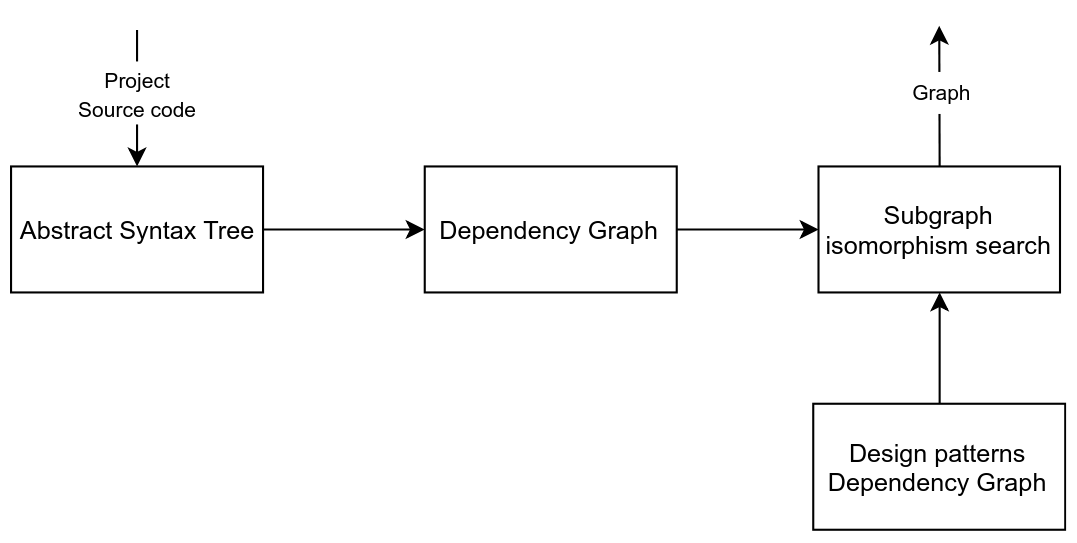
\includegraphics[scale=0.36]{images/general_architecture_3_1}
	\caption{Quá trình kiểm tra sự tuân thủ mẫu thiết kế của mã nguồn}
	\label{fig:universe}
\end{figure}
\section{Tiền xử lý mã nguồn Java}
\textbf{Định nghĩa:} (\textit{Cây cấu trúc} \cite{jcia}) đối với mã nguồn Java. Là một cây cấu trúc với $T = (N,E)$ với $N =  \{n_1,n_2,n_3...n_k\}$ là tập hợp các nút trên cây, mỗi nút đại diện cho một thành phần của mã nguồn ví dụ như thư mục, tệp, lớp, phương thức,... $R = \{(v_i,v_j)|v_i \in N \and v_j in N  \}$ là tập hợp các cặp hai đỉnh không sắp thứ tự, mỗi cặp đỉnh tương ứng với một cạnh ký hiện $n_in_j$ tức là $n_i$ và $n_j$ là hai đỉnh kề.

\newpage
\section{Phân tích cấu trúc mã nguồn}
\subsection{Phân tích phụ thuộc giữa các thành phần trong mã nguồn}
\subsection{Xây dựng đồ thị phụ thuộc từ cây cấu trúc}
\subsection{Ví dụ minh họa}

\newpage
\section{Kiểm tra sự tuân thủ mẫu thiết kế bên trong mã nguồn}

\begin{thebibliography}{9}
	\section*{Tiếng Việt}
	
	\section*{Tiếng Anh}
	\bibitem{jcia}
	Ba Cuong Le, Son Nguyen Van, Duc Anh Nguyen, Ngoc Hung Pham, Hieu Vo Dinh. JCIA: A Tool for Change Impact Analysis of Java EE Applications. Information Systems Design and Intelligent Applications, pp.105-114, 2018.
	
	
\end{thebibliography}



\end{document}
